\documentclass{arxivtmpl}

%%%%%%%%%%%%%%%%%%%%%%%%%%%%%%%%%%%%%%%%%%%%%%%%%%%%%%%%%%%%%%%%%%%%%%%%%%%%%%%%%%%%%%%%%%%%%%%%%%%%%%%%%%%%%%%%%%
%%  Part 1: dlbook 数学记法（random / vector / matrix / tensor / graph / set / 算子）
%%%%%%%%%%%%%%%%%%%%%%%%%%%%%%%%%%%%%%%%%%%%%%%%%%%%%%%%%%%%%%%%%%%%%%%%%%%%%%%%%%%%%%%%%%%%%%%%%%%%%%%%%%%%%%%%%%

% Mark sections of captions for referring to divisions of figures
\newcommand{\figleft}{{\em (Left)}}
\newcommand{\figcenter}{{\em (Center)}}
\newcommand{\figright}{{\em (Right)}}
\newcommand{\figtop}{{\em (Top)}}
\newcommand{\figbottom}{{\em (Bottom)}}
\newcommand{\captiona}{{\em (a)}}
\newcommand{\captionb}{{\em (b)}}
\newcommand{\captionc}{{\em (c)}}
\newcommand{\captiond}{{\em (d)}}

% Highlight a newly defined term
\newcommand{\newterm}[1]{{\bf #1}}


\def\ceil#1{\lceil #1 \rceil}
\def\floor#1{\lfloor #1 \rfloor}
\def\1{\bm{1}}
\newcommand{\train}{\mathcal{D}}
\newcommand{\valid}{\mathcal{D_{\mathrm{valid}}}}
\newcommand{\test}{\mathcal{D_{\mathrm{test}}}}

\def\eps{{\epsilon}}


% Random variables
\def\reta{{\textnormal{$\eta$}}}
\def\ra{{\textnormal{a}}}
\def\rb{{\textnormal{b}}}
\def\rc{{\textnormal{c}}}
\def\rd{{\textnormal{d}}}
\def\re{{\textnormal{e}}}
\def\rf{{\textnormal{f}}}
\def\rg{{\textnormal{g}}}
\def\rh{{\textnormal{h}}}
\def\ri{{\textnormal{i}}}
\def\rj{{\textnormal{j}}}
\def\rk{{\textnormal{k}}}
\def\rl{{\textnormal{l}}}
% rm is already a command, just don't name any random variables m
\def\rn{{\textnormal{n}}}
\def\ro{{\textnormal{o}}}
\def\rp{{\textnormal{p}}}
\def\rq{{\textnormal{q}}}
\def\rr{{\textnormal{r}}}
\def\rs{{\textnormal{s}}}
\def\rt{{\textnormal{t}}}
\def\ru{{\textnormal{u}}}
\def\rv{{\textnormal{v}}}
\def\rw{{\textnormal{w}}}
\def\rx{{\textnormal{x}}}
\def\ry{{\textnormal{y}}}
\def\rz{{\textnormal{z}}}

% Random vectors
\def\rvepsilon{{\mathbf{\epsilon}}}
\def\rvtheta{{\mathbf{\theta}}}
\def\rva{{\mathbf{a}}}
\def\rvb{{\mathbf{b}}}
\def\rvc{{\mathbf{c}}}
\def\rvd{{\mathbf{d}}}
\def\rve{{\mathbf{e}}}
\def\rvf{{\mathbf{f}}}
\def\rvg{{\mathbf{g}}}
\def\rvh{{\mathbf{h}}}
\def\rvi{{\mathbf{i}}}
\def\rvj{{\mathbf{j}}}
\def\rvk{{\mathbf{k}}}
\def\rvl{{\mathbf{l}}}
\def\rvm{{\mathbf{m}}}
\def\rvn{{\mathbf{n}}}
\def\rvo{{\mathbf{o}}}
\def\rvp{{\mathbf{p}}}
\def\rvq{{\mathbf{q}}}
\def\rvr{{\mathbf{r}}}
\def\rvs{{\mathbf{s}}}
\def\rvt{{\mathbf{t}}}
\def\rvu{{\mathbf{u}}}
\def\rvv{{\mathbf{v}}}
\def\rvw{{\mathbf{w}}}
\def\rvx{{\mathbf{x}}}
\def\rvy{{\mathbf{y}}}
\def\rvz{{\mathbf{z}}}

% Elements of random vectors
\def\erva{{\textnormal{a}}}
\def\ervb{{\textnormal{b}}}
\def\ervc{{\textnormal{c}}}
\def\ervd{{\textnormal{d}}}
\def\erve{{\textnormal{e}}}
\def\ervf{{\textnormal{f}}}
\def\ervg{{\textnormal{g}}}
\def\ervh{{\textnormal{h}}}
\def\ervi{{\textnormal{i}}}
\def\ervj{{\textnormal{j}}}
\def\ervk{{\textnormal{k}}}
\def\ervl{{\textnormal{l}}}
\def\ervm{{\textnormal{m}}}
\def\ervn{{\textnormal{n}}}
\def\ervo{{\textnormal{o}}}
\def\ervp{{\textnormal{p}}}
\def\ervq{{\textnormal{q}}}
\def\ervr{{\textnormal{r}}}
\def\ervs{{\textnormal{s}}}
\def\ervt{{\textnormal{t}}}
\def\ervu{{\textnormal{u}}}
\def\ervv{{\textnormal{v}}}
\def\ervw{{\textnormal{w}}}
\def\ervx{{\textnormal{x}}}
\def\ervy{{\textnormal{y}}}
\def\ervz{{\textnormal{z}}}

% Random matrices
\def\rmA{{\mathbf{A}}}
\def\rmB{{\mathbf{B}}}
\def\rmC{{\mathbf{C}}}
\def\rmD{{\mathbf{D}}}
\def\rmE{{\mathbf{E}}}
\def\rmF{{\mathbf{F}}}
\def\rmG{{\mathbf{G}}}
\def\rmH{{\mathbf{H}}}
\def\rmI{{\mathbf{I}}}
\def\rmJ{{\mathbf{J}}}
\def\rmK{{\mathbf{K}}}
\def\rmL{{\mathbf{L}}}
\def\rmM{{\mathbf{M}}}
\def\rmN{{\mathbf{N}}}
\def\rmO{{\mathbf{O}}}
\def\rmP{{\mathbf{P}}}
\def\rmQ{{\mathbf{Q}}}
\def\rmR{{\mathbf{R}}}
\def\rmS{{\mathbf{S}}}
\def\rmT{{\mathbf{T}}}
\def\rmU{{\mathbf{U}}}
\def\rmV{{\mathbf{V}}}
\def\rmW{{\mathbf{W}}}
\def\rmX{{\mathbf{X}}}
\def\rmY{{\mathbf{Y}}}
\def\rmZ{{\mathbf{Z}}}

% Elements of random matrices
\def\ermA{{\textnormal{A}}}
\def\ermB{{\textnormal{B}}}
\def\ermC{{\textnormal{C}}}
\def\ermD{{\textnormal{D}}}
\def\ermE{{\textnormal{E}}}
\def\ermF{{\textnormal{F}}}
\def\ermG{{\textnormal{G}}}
\def\ermH{{\textnormal{H}}}
\def\ermI{{\textnormal{I}}}
\def\ermJ{{\textnormal{J}}}
\def\ermK{{\textnormal{K}}}
\def\ermL{{\textnormal{L}}}
\def\ermM{{\textnormal{M}}}
\def\ermN{{\textnormal{N}}}
\def\ermO{{\textnormal{O}}}
\def\ermP{{\textnormal{P}}}
\def\ermQ{{\textnormal{Q}}}
\def\ermR{{\textnormal{R}}}
\def\ermS{{\textnormal{S}}}
\def\ermT{{\textnormal{T}}}
\def\ermU{{\textnormal{U}}}
\def\ermV{{\textnormal{V}}}
\def\ermW{{\textnormal{W}}}
\def\ermX{{\textnormal{X}}}
\def\ermY{{\textnormal{Y}}}
\def\ermZ{{\textnormal{Z}}}

% Vectors
\def\vzero{{\bm{0}}}
\def\vone{{\bm{1}}}
\def\vmu{{\bm{\mu}}}
\def\vtheta{{\bm{\theta}}}
\def\va{{\bm{a}}}
\def\vb{{\bm{b}}}
\def\vc{{\bm{c}}}
\def\vd{{\bm{d}}}
\def\ve{{\bm{e}}}
\def\vf{{\bm{f}}}
\def\vg{{\bm{g}}}
\def\vh{{\bm{h}}}
\def\vi{{\bm{i}}}
\def\vj{{\bm{j}}}
\def\vk{{\bm{k}}}
\def\vl{{\bm{l}}}
\def\vm{{\bm{m}}}
\def\vn{{\bm{n}}}
\def\vo{{\bm{o}}}
\def\vp{{\bm{p}}}
\def\vq{{\bm{q}}}
\def\vr{{\bm{r}}}
\def\vs{{\bm{s}}}
\def\vt{{\bm{t}}}
\def\vu{{\bm{u}}}
\def\vv{{\bm{v}}}
\def\vw{{\bm{w}}}
\def\vx{{\bm{x}}}
\def\vy{{\bm{y}}}
\def\vz{{\bm{z}}}

% Elements of vectors
\def\evalpha{{\alpha}}
\def\evbeta{{\beta}}
\def\evepsilon{{\epsilon}}
\def\evlambda{{\lambda}}
\def\evomega{{\omega}}
\def\evmu{{\mu}}
\def\evpsi{{\psi}}
\def\evsigma{{\sigma}}
\def\evtheta{{\theta}}
\def\eva{{a}}
\def\evb{{b}}
\def\evc{{c}}
\def\evd{{d}}
\def\eve{{e}}
\def\evf{{f}}
\def\evg{{g}}
\def\evh{{h}}
\def\evi{{i}}
\def\evj{{j}}
\def\evk{{k}}
\def\evl{{l}}
\def\evm{{m}}
\def\evn{{n}}
\def\evo{{o}}
\def\evp{{p}}
\def\evq{{q}}
\def\evr{{r}}
\def\evs{{s}}
\def\evt{{t}}
\def\evu{{u}}
\def\evv{{v}}
\def\evw{{w}}
\def\evx{{x}}
\def\evy{{y}}
\def\evz{{z}}

% Matrix
\def\mA{{\bm{A}}}
\def\mB{{\bm{B}}}
\def\mC{{\bm{C}}}
\def\mD{{\bm{D}}}
\def\mE{{\bm{E}}}
\def\mF{{\bm{F}}}
\def\mG{{\bm{G}}}
\def\mH{{\bm{H}}}
\def\mI{{\bm{I}}}
\def\mJ{{\bm{J}}}
\def\mK{{\bm{K}}}
\def\mL{{\bm{L}}}
\def\mM{{\bm{M}}}
\def\mN{{\bm{N}}}
\def\mO{{\bm{O}}}
\def\mP{{\bm{P}}}
\def\mQ{{\bm{Q}}}
\def\mR{{\bm{R}}}
\def\mS{{\bm{S}}}
\def\mT{{\bm{T}}}
\def\mU{{\bm{U}}}
\def\mV{{\bm{V}}}
\def\mW{{\bm{W}}}
\def\mX{{\bm{X}}}
\def\mY{{\bm{Y}}}
\def\mZ{{\bm{Z}}}
\def\mBeta{{\bm{\beta}}}
\def\mPhi{{\bm{\Phi}}}
\def\mLambda{{\bm{\Lambda}}}
\def\mSigma{{\bm{\Sigma}}}

% Tensor
\DeclareMathAlphabet{\mathsfit}{\encodingdefault}{\sfdefault}{m}{sl}
\SetMathAlphabet{\mathsfit}{bold}{\encodingdefault}{\sfdefault}{bx}{n}
\newcommand{\tens}[1]{\bm{\mathsfit{#1}}}
\def\tA{{\tens{A}}}
\def\tB{{\tens{B}}}
\def\tC{{\tens{C}}}
\def\tD{{\tens{D}}}
\def\tE{{\tens{E}}}
\def\tF{{\tens{F}}}
\def\tG{{\tens{G}}}
\def\tH{{\tens{H}}}
\def\tI{{\tens{I}}}
\def\tJ{{\tens{J}}}
\def\tK{{\tens{K}}}
\def\tL{{\tens{L}}}
\def\tM{{\tens{M}}}
\def\tN{{\tens{N}}}
\def\tO{{\tens{O}}}
\def\tP{{\tens{P}}}
\def\tQ{{\tens{Q}}}
\def\tR{{\tens{R}}}
\def\tS{{\tens{S}}}
\def\tT{{\tens{T}}}
\def\tU{{\tens{U}}}
\def\tV{{\tens{V}}}
\def\tW{{\tens{W}}}
\def\tX{{\tens{X}}}
\def\tY{{\tens{Y}}}
\def\tZ{{\tens{Z}}}


% Graph
\def\gA{{\mathcal{A}}}
\def\gB{{\mathcal{B}}}
\def\gC{{\mathcal{C}}}
\def\gD{{\mathcal{D}}}
\def\gE{{\mathcal{E}}}
\def\gF{{\mathcal{F}}}
\def\gG{{\mathcal{G}}}
\def\gH{{\mathcal{H}}}
\def\gI{{\mathcal{I}}}
\def\gJ{{\mathcal{J}}}
\def\gK{{\mathcal{K}}}
\def\gL{{\mathcal{L}}}
\def\gM{{\mathcal{M}}}
\def\gN{{\mathcal{N}}}
\def\gO{{\mathcal{O}}}
\def\gP{{\mathcal{P}}}
\def\gQ{{\mathcal{Q}}}
\def\gR{{\mathcal{R}}}
\def\gS{{\mathcal{S}}}
\def\gT{{\mathcal{T}}}
\def\gU{{\mathcal{U}}}
\def\gV{{\mathcal{V}}}
\def\gW{{\mathcal{W}}}
\def\gX{{\mathcal{X}}}
\def\gY{{\mathcal{Y}}}
\def\gZ{{\mathcal{Z}}}

% Sets
\def\sA{{\mathbb{A}}}
\def\sB{{\mathbb{B}}}
\def\sC{{\mathbb{C}}}
\def\sD{{\mathbb{D}}}
% Don't use a set called E, because this would be the same as our symbol
% for expectation.
\def\sF{{\mathbb{F}}}
\def\sG{{\mathbb{G}}}
\def\sH{{\mathbb{H}}}
\def\sI{{\mathbb{I}}}
\def\sJ{{\mathbb{J}}}
\def\sK{{\mathbb{K}}}
\def\sL{{\mathbb{L}}}
\def\sM{{\mathbb{M}}}
\def\sN{{\mathbb{N}}}
\def\sO{{\mathbb{O}}}
\def\sP{{\mathbb{P}}}
\def\sQ{{\mathbb{Q}}}
\def\sR{{\mathbb{R}}}
\def\sS{{\mathbb{S}}}
\def\sT{{\mathbb{T}}}
\def\sU{{\mathbb{U}}}
\def\sV{{\mathbb{V}}}
\def\sW{{\mathbb{W}}}
\def\sX{{\mathbb{X}}}
\def\sY{{\mathbb{Y}}}
\def\sZ{{\mathbb{Z}}}

% Entries of a matrix
\def\emLambda{{\Lambda}}
\def\emA{{A}}
\def\emB{{B}}
\def\emC{{C}}
\def\emD{{D}}
\def\emE{{E}}
\def\emF{{F}}
\def\emG{{G}}
\def\emH{{H}}
\def\emI{{I}}
\def\emJ{{J}}
\def\emK{{K}}
\def\emL{{L}}
\def\emM{{M}}
\def\emN{{N}}
\def\emO{{O}}
\def\emP{{P}}
\def\emQ{{Q}}
\def\emR{{R}}
\def\emS{{S}}
\def\emT{{T}}
\def\emU{{U}}
\def\emV{{V}}
\def\emW{{W}}
\def\emX{{X}}
\def\emY{{Y}}
\def\emZ{{Z}}
\def\emSigma{{\Sigma}}

% entries of a tensor
% Same font as tensor, without \bm wrapper
\newcommand{\etens}[1]{\mathsfit{#1}}
\def\etLambda{{\etens{\Lambda}}}
\def\etA{{\etens{A}}}
\def\etB{{\etens{B}}}
\def\etC{{\etens{C}}}
\def\etD{{\etens{D}}}
\def\etE{{\etens{E}}}
\def\etF{{\etens{F}}}
\def\etG{{\etens{G}}}
\def\etH{{\etens{H}}}
\def\etI{{\etens{I}}}
\def\etJ{{\etens{J}}}
\def\etK{{\etens{K}}}
\def\etL{{\etens{L}}}
\def\etM{{\etens{M}}}
\def\etN{{\etens{N}}}
\def\etO{{\etens{O}}}
\def\etP{{\etens{P}}}
\def\etQ{{\etens{Q}}}
\def\etR{{\etens{R}}}
\def\etS{{\etens{S}}}
\def\etT{{\etens{T}}}
\def\etU{{\etens{U}}}
\def\etV{{\etens{V}}}
\def\etW{{\etens{W}}}
\def\etX{{\etens{X}}}
\def\etY{{\etens{Y}}}
\def\etZ{{\etens{Z}}}

% The true underlying data generating distribution
\newcommand{\pdata}{p_{\rm{data}}}
% The empirical distribution defined by the training set
\newcommand{\ptrain}{\hat{p}_{\rm{data}}}
\newcommand{\Ptrain}{\hat{P}_{\rm{data}}}
% The model distribution
\newcommand{\pmodel}{p_{\rm{model}}}
\newcommand{\Pmodel}{P_{\rm{model}}}
\newcommand{\ptildemodel}{\tilde{p}_{\rm{model}}}
% Stochastic autoencoder distributions
\newcommand{\pencode}{p_{\rm{encoder}}}
\newcommand{\pdecode}{p_{\rm{decoder}}}
\newcommand{\precons}{p_{\rm{reconstruct}}}

\newcommand{\laplace}{\mathrm{Laplace}}

\newcommand{\R}{\mathbb{R}}
\newcommand{\E}{\mathbb{E}}
\newcommand{\Ls}{\mathcal{L}}
\newcommand{\emp}{\tilde{p}}
\newcommand{\lr}{\alpha}
\newcommand{\reg}{\lambda}
\newcommand{\rect}{\mathrm{rectifier}}
\newcommand{\softmax}{\mathrm{softmax}}
\newcommand{\sigmoid}{\sigma}
\newcommand{\softplus}{\zeta}
\newcommand{\standarderror}{\mathrm{SE}}
\newcommand{\normlzero}{L^0}
\newcommand{\normlone}{L^1}
\newcommand{\normltwo}{L^2}
\newcommand{\normlp}{L^p}
\newcommand{\normmax}{L^\infty}

\newcommand{\parents}{Pa}

\DeclareMathOperator*{\argmax}{arg\,max}
\DeclareMathOperator*{\argmin}{arg\,min}

\DeclareMathOperator{\sign}{sign}
\DeclareMathOperator{\Tr}{Tr}
\let\ab\allowbreak

%%%%%%%%%%%%%%%%%%%%%%%%%%%%%%%%%%%%%%%%%%%%%%%%%%%%%%%%%%%%%%%%%%%%%%%%%%%%%%%%%%%%%%%%%%%%%%%%%%%%%%%%%%%%%%%%%%
%%  Part 2: callout / listing / teaser / 批注 / hyperref / 表格配色 / algorithm2e
%%%%%%%%%%%%%%%%%%%%%%%%%%%%%%%%%%%%%%%%%%%%%%%%%%%%%%%%%%%%%%%%%%%%%%%%%%%%%%%%%%%%%%%%%%%%%%%%%%%%%%%%%%%%%%%%%%


%% ---- Callout family (tcolorbox): frameless, light palette tint + 3pt left accent bar ----
%% \finding{n}{text} / \note{text} / \tip{text} / \warning{text} share one look; only the
%% palette color changes. Labels use the accent color, except \warning (black label, since
%% yellow text is unreadable and the palette forbids darkening toward black).
\tcbuselibrary{skins,breakable}
\newtcolorbox{findingbox}{enhanced,breakable,frame hidden,colback=gred!6,borderline west={3pt}{0pt}{gred},sharp corners,boxsep=0pt,left=12pt,right=10pt,top=8pt,bottom=8pt,before skip=12pt,after skip=12pt}
\newtcolorbox{notebox}{enhanced,breakable,frame hidden,colback=gblue!6,borderline west={3pt}{0pt}{gblue},sharp corners,boxsep=0pt,left=12pt,right=10pt,top=8pt,bottom=8pt,before skip=12pt,after skip=12pt}
\newtcolorbox{tipbox}{enhanced,breakable,frame hidden,colback=ggreen!6,borderline west={3pt}{0pt}{ggreen},sharp corners,boxsep=0pt,left=12pt,right=10pt,top=8pt,bottom=8pt,before skip=12pt,after skip=12pt}
\newtcolorbox{warnbox}{enhanced,breakable,frame hidden,colback=gyellow!6,borderline west={3pt}{0pt}{gyellow},sharp corners,boxsep=0pt,left=12pt,right=10pt,top=8pt,bottom=8pt,before skip=12pt,after skip=12pt}
\newcommand{\finding}[2]{\begin{findingbox}{\sffamily\bfseries\color{gred}Finding~#1.}\ #2\end{findingbox}}
\newcommand{\note}[1]{\begin{notebox}{\sffamily\bfseries\color{gblue}Note.}\ #1\end{notebox}}
\newcommand{\tip}[1]{\begin{tipbox}{\sffamily\bfseries\color{ggreen}Tip.}\ #1\end{tipbox}}
\newcommand{\warning}[1]{\begin{warnbox}{\sffamily\bfseries Warning.}\ #1\end{warnbox}}

%% ---- Global listing defaults (promptbox) ----
\tcbuselibrary{listings}
%% 字号用 \fontsize 绝对值：\footnotesize 会让 listings 与正文各取不同 optical size（9.96 vs 8.97）
\newcommand{\boxfont}{\fontsize{9}{11}\selectfont}
\lstset{
  basicstyle=\ttfamily\boxfont,
  breaklines=true, breakindent=0pt, breakautoindent=false,
  columns=fullflexible, keepspaces=true,
  xleftmargin=0pt, xrightmargin=0pt, resetmargins=true,
  aboveskip=0pt, belowskip=0pt,
}
%% 段间距：listings 没有"段距"参数，段落用空行分隔；一个空行 = 此高度的间距。
\newcommand{\lstparskip}{0.5\baselineskip}        % listing / transcript 段落间距，全局可调
\newcommand{\lstgap}{\vspace{\lstparskip}}        % promptbox 内段落分隔：写 (*\lstgap*) 注入此间距（靠 escapeinside）
%% ---- Prompt box: callout look (left accent + light tint, like \note) with a verbatim listing body ----
%% \begin{promptbox}[System|User|Prompt] ...verbatim text... \end{promptbox}  (palette: gblue)
\newtcblisting{promptbox}[1][]{%
  enhanced, listing only, breakable, frame hidden, width=\linewidth,
  colback=gblue!6, borderline west={3pt}{0pt}{gblue},
  sharp corners, boxsep=0pt,
  left=12pt, right=10pt, top=8pt, bottom=8pt, before skip=12pt, after skip=12pt,
  before upper={\def\promptlabel{#1}\ifx\promptlabel\empty\else{\sffamily\bfseries\color{gblue}#1}\par\smallskip\fi},   % optional label; empty => no in-box label (use a \section instead)
  listing options={basicstyle=\ttfamily\boxfont, escapeinside={(*}{*)}},
}

%% ---- Transcript box: green callout for a multi-turn agent trace; \speaker{User|Assistant|Tool} per turn ----
\newtcolorbox{transcriptbox}{%
  enhanced, breakable, frame hidden,
  colback=ggreen!6, borderline west={3pt}{0pt}{ggreen},
  sharp corners, boxsep=0pt, fontupper=\ttfamily\boxfont, halign upper=flush left,   % monospace body, same size as the listing font
  left=12pt, right=10pt, top=6pt, bottom=8pt, before skip=12pt, after skip=12pt,
}
\newcommand{\speaker}[1]{\par\addvspace{\lstparskip}\noindent{\sffamily\bfseries\color{ggreen}#1:}\hspace{0.6em}\ignorespaces}

%% ---- Teaser figure: full-width hero figure + numbered caption, for page 1 ----
%% \teaserfigure{<graphics>}{<caption>} ; \teaserplaceholder = a stand-in grey box.
\newcommand{\teaserplaceholder}{%
  \fcolorbox{ggrey!40}{ggrey!8}{\parbox[c][6.5cm][c]{\dimexpr\linewidth-2\fboxsep-2\fboxrule\relax}{\centering\sffamily\color{ggrey!80}[\,teaser figure placeholder\,]}}%
}
\newcommand{\teaserfigure}[2]{%
  \begingroup\centering\captionsetup{type=figure}
  #1\par\vspace{0.4em}\caption{#2}%
  \par\endgroup\vspace{1em}
}

%% ---- Code block: yellow listing callout, python lexer ----
%% \begin{codebox} ...verbatim... \end{codebox}  (palette: gyellow)
%% codebox uses minted directly (pygments). tcolorbox+minted (tcblisting) mishandles '#',
%% so the yellow-callout look comes from minted's own frame + bgcolor.
\colorlet{codebg}{gyellow!6}
\setminted{fontsize=\boxfont, breaklines, autogobble, tabsize=4, style=vs}
\newminted[codebox]{python}{bgcolor=codebg, frame=leftline, framerule=2.5pt, rulecolor=gyellow, framesep=2.5mm}


\newcommand{\ensuretext}[1]{#1}
\newcommand{\marker}[2]{\ensuremath{^{\textsc{#1}}_{\textsc{#2}}}}
\newcommand{\arkcomment}[3]{\ensuretext{\textcolor{#3}{[#1 #2]}}}
\newcommand{\wchai}[1]{\arkcomment{\marker{W.H.}{Chai}}{#1}{gpurple}}

%% hyperref：链接统一 linkcol（gblue）文字色，无边框
\hypersetup{
    colorlinks=true,
    linkcolor=linkcol,
    citecolor=linkcol,
    urlcolor=linkcol,
    pdfborderstyle={},
    pdfborder={0 0 0}
}
\bibliographystyle{unsrt}

%% 作者 / 机构：Lato sans（与章节标题同族）；作者 bold，机构 regular
\renewcommand\Authfont{\sffamily\bfseries}
\renewcommand\Affilfont{\sffamily\mdseries}

%% ---- Leaderboard 表配色（单色热力图 perf0..perf80，基色 = palette blue）----
\colorlet{perfhue}{gblue}
\colorlet{perf0}{white}
\colorlet{perf10}{perfhue!12}
\colorlet{perf20}{perfhue!22}
\colorlet{perf30}{perfhue!33}
\colorlet{perf40}{perfhue!44}
\colorlet{perf50}{perfhue!55}
\colorlet{perf60}{perfhue!66}
\colorlet{perf70}{perfhue!77}
\colorlet{perf80}{perfhue!88}

\newcommand{\blackcircle}{
~{\leavevmode\put(0,2.83){\circle*{5.5}}}~
}




\newcommand{\RN}[1]{%
	\textup{\lowercase\expandafter{\it \romannumeral#1}}%
}

\def\Dir{\textsf{Dir}}
\def\Bern{\textsf{Ber}}
\def\Pois{\textsf{Pois}}
\def\Std{\textsf{Std}}
\def\Var{\textsf{Var}}
\def\Cor{\textsf{Cor}}
\def\Cov{\textsf{Cov}}
\def\Gal{\textsf{Gamma}}
\def\Beta{\textsf{Beta}}
\def\KL{\textsf{KL}}
\def\VI{\textsf{VI}}
\def\MI{\textsf{MI}}
\def\Ent{\textsf{H}} %entropy; \H is LaTeX's accent (Erd\H{o}s), do not redefine

\newcommand{\ie}[0]{\emph{i.e., }}
\newcommand{\ea}[0]{\emph{et al. }}
\newcommand{\eg}[0]{\emph{e.g., }}
\newcommand{\cf}[0]{\emph{cf. }}
\newcommand{\etc}[0]{\emph{etc.}}

\newcommand\blfootnote[1]{%
  \begingroup
  \renewcommand\thefootnote{}\footnote{#1}%
  \addtocounter{footnote}{-1}%
  \endgroup
}

\newcommand{\cmark}{\ding{51}}%
\newcommand{\xmark}{\ding{55}}%

\newcommand*\circled[1]{\tikz[baseline=(char.base)]{
            \node[shape=circle,draw,inner sep=0.6pt] (char) {#1};}}

\newcommand{\std}[1]{\,{\tiny $\pm$ #1}}       % 均值后跟小号 ±std：83.1\std{0.4}；\tiny 限在组内，prose 里可用
\newcommand{\default}[1]{\cellcolor{ggrey!15}#1}   % ablation 表 default 配置的 cell（灰底）
\newtheorem{assumption}{Assumption}   % cls 没有 assumption，Method 理论型要用

\SetKwInput{KwInput}{Input}
\SetKwInput{KwOutput}{Output}
\DontPrintSemicolon


% Define pseudocode formatting
\renewcommand{\KwSty}[1]{\textnormal{\textcolor{gblue}{\ttfamily\bfseries #1}}\unskip}
\renewcommand{\ArgSty}[1]{\textnormal{\ttfamily #1}\unskip}
\SetKwComment{Comment}{\color{ggreen}\# }{}
\renewcommand{\CommentSty}[1]{\textnormal{\ttfamily\color{ggreen}#1}\unskip}
\newcommand{\assign}{\leftarrow}
\newcommand{\var}{\texttt}
\newcommand{\FuncCall}[2]{\texttt{\bfseries #1(#2)}}
\SetKwProg{Function}{def}{:}{}
\renewcommand{\ProgSty}[1]{\texttt{\bfseries #1}}
\SetKwProg{For}{for}{:}{}
\SetKwProg{If}{if}{:}{}
\newcommand{\VarSty}[1]{\textnormal{\ttfamily\color{gblue}#1}\unskip}
\newcommand{\PredSty}[1]{\textnormal{\ttfamily\color{ggreen}#1}\unskip}


\graphicspath{{../figures/}}
\newcolumntype{L}{>{\raggedright\arraybackslash}X}
\DeclareUnicodeCharacter{03B3}{\ensuremath{\gamma}}
\DeclareUnicodeCharacter{03BB}{\ensuremath{\lambda}}
\DeclareUnicodeCharacter{03BC}{\ensuremath{\mu}}
\DeclareUnicodeCharacter{03C1}{\ensuremath{\rho}}
\DeclareUnicodeCharacter{2032}{\ensuremath{'}}
\DeclareUnicodeCharacter{2081}{\ensuremath{_1}}
\DeclareUnicodeCharacter{2212}{\ensuremath{-}}

\title{Influence Between Agents in the AI Village}

\author[1]{Enxin Song}
\author[2]{Wenhao Chai}
\affil[1]{University of Pennsylvania}
\affil[2]{Princeton University}

\begin{document}

\maketitle

\thispagestyle{firstpagestyle}

\begin{abstract}
{\sffamily\fontseries{eb}\normalsize\selectfont Abstract}\par\vspace{0.15\baselineskip}
\small
Agents in the AI Village influence each other through chat, information and shared work, but in chat and work each agent mostly continues its own activity. Self-excitation triggers 47.5\% of agent messages, more than any other source, and cascades of messages between agents die out in 39 of 42 goal windows. Information retold between agents reaches fewer agents than the population allows, travels more slowly with each retelling and changes along the way. Each agent loses about a third of new facts at its first memory consolidation, and the facts that survive grow safer. Six in ten computer-use sessions that build on earlier work continue the agent's own previous session. Behavioural change points do not line up with documented scaffolding changes beyond chance.
\end{abstract}

\teaserfigure{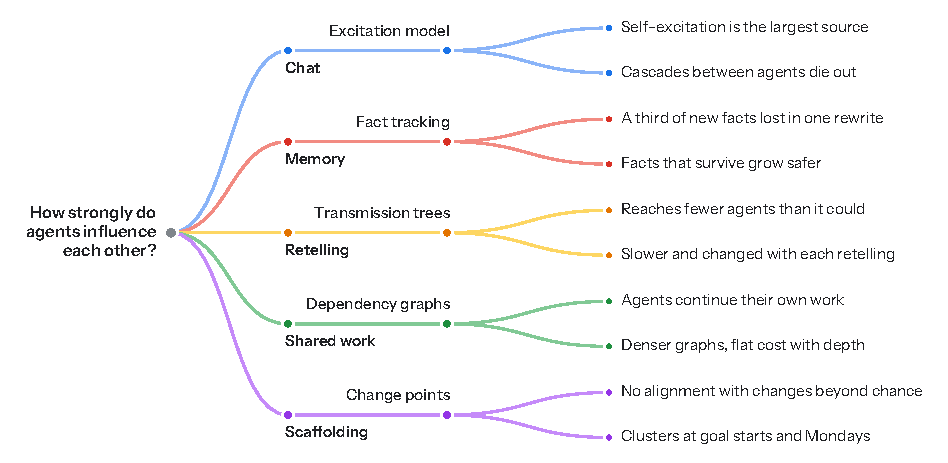
\includegraphics[width=\linewidth]{overview.pdf}}{The core question, the five questions under it, the method for each and its two main findings, read from left to right. Each branch is one of Sections 3 to 7.}

\clearpage
\section{Introduction}

We ask how strongly LLM agents influence each other when they share a chat, a memory scaffold and a stream of goals for a year and a half. We answer it on the AI Village logs with avsd, a toolkit that turns them into one unified event table. Figure 1 splits the question into five, each answered by one method. An excitation model asks who triggers whom in the chat, and fact tracking asks how long facts survive in each agent's own memory. Transmission trees follow information retold between agents, dependency graphs follow shared work, and change-point detection asks whether documented scaffolding changes shift behaviour.

\setcounter{tocdepth}{2}
\begingroup
\hypersetup{linkcolor=black}
\tableofcontents
\endgroup
\clearpage

\section{Data}

We use the AI Village dataset of AI Digest (2026) at Hugging Face revision 838b4150. It covers 46 agents from 2025-04-02 to 2026-09-18, more than the dataset card lists, and Table A1 gives the size of each table. Every analysis here uses the logs, so we did not download the 171.1 GB of screenshots.

We merge six sources into one event table of 3.2 million rows that reconciles with every source table. Each row carries UTC and Pacific times and an actor type of agent, human or system. Run days are the 389 Pacific dates with activity, and active time leaves out pauses longer than 30 minutes. The roster holds four model families, and we analyse the Claude Code agent apart because it runs a different scaffold. The CHANGELOG yields 186 dated scaffolding and roster entries.

Humans appear only as the category human, and no output carries names, emails, phone numbers or message text. Credentials left in the logs were recorded by location only and never used.

\section{Chat}

Who triggers whom in the chat?

\subsection{Method}

We model agent chat as a multivariate Hawkes process, with one dimension per agent and one realization per run block. The intensity of agent i at time t since the block start is
\[ \lambda_i(t) = \mu_{i,b(t)} + \sum_j \sum_{t_l < t} n_{ij}\, g_{c(i,j)}(t - t_l), \]
with a baseline μ over eight hourly bins b(t) and a branching ratio $n_{ij}$ from source j. The sources are the agent itself, other agents, humans and the scaffold's bot. Each kernel $g_c$ mixes exponentials with time scales from 1 minute to 1 hour (Veen and Schoenberg 2008). An agent counts only on realizations where it is present in its room, and we fit by expectation maximisation.

Windows follow the 51 village goals and take their names from them, so G35-39 covers goals 35 to 39. A recovery check refits simulations of each window, and 42 of the final 43 windows pass. The spectral radius ρ of the agent-to-agent part tells whether cascades of messages grow or die out, with ρ below 1 meaning that they die out.

\subsection{Findings}

Self-excitation is the largest source of agent messages. Over the 43 windows it triggers 47.5\% of agent messages, against 25.9\% for the baseline, 23.8\% for other agents and under 2\% each for humans and the scaffold. As shown in Figure 2, self-excitation leads in 24 of the 42 accepted windows. The baseline dominates from December 2025 to March 2026, and humans trigger more messages only while the chat was public.

\begin{figure}[htbp]
\centering
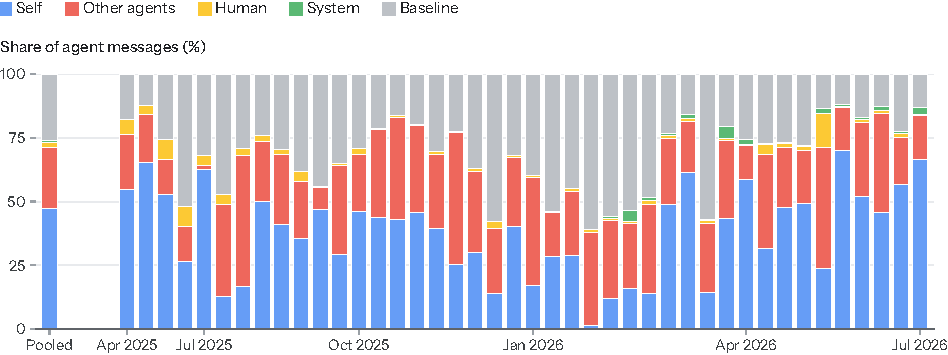
\includegraphics[width=\linewidth]{sources.pdf}
\caption{Share of agent messages by triggering source in the excitation model, event-weighted over the 43 goal windows in the first bar and then for each of the 42 accepted windows by start date. Self-excitation is the largest source in 24 of the 42 windows, and the baseline exceeds half in six windows between December 2025 and March 2026.}
\end{figure}

Cascades between agents die out in almost every window once absence is modelled. As shown in Figure 3, ρ is below 1 in 39 of the 42 accepted windows, and no bootstrap interval lies wholly above 1. Treating absent agents as present pushes ρ above 1 in 17 of 44 windows, because the fit turns the bursts of part-time agents into self-excitation.

\begin{figure}[htbp]
\centering
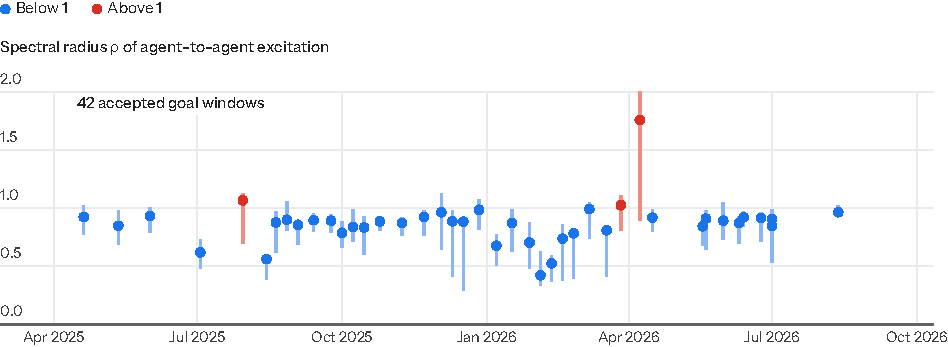
\includegraphics[width=\linewidth]{rho.pdf}
\caption{Spectral radius ρ of agent-to-agent excitation in each accepted goal window, at the window's midpoint, with run-date bootstrap 95\% intervals cut at 2. Cascades of agent messages die out when ρ lies below 1, as it does in 39 of the 42 windows.}
\end{figure}

The model recovers the shares of simulated windows but fits the timing of single agents poorly. Time-rescaling (Brown et al. 2002) rejects in 68\% of agent dimensions, and the most probable parent of a message matches explicit name references less often than the latest message by someone else. Near findings of the AI Digest LLM monitor, the model attributes more of the involved agents' messages to their own earlier messages. Flagged pairs rank high in coupling, mostly because a few pairs are flagged again and again.

\section{Memory}

How long do facts survive in an agent's own memory?

\subsection{Method}

Each memory row is a full snapshot, and a consolidation is a row that rewrites the previous version. The scaffold prompts every rewrite, both at regular consolidation steps and when the memory exceeds a length cap (Binksmith 2026). We follow fact units, rule-extracted anchors such as URLs, numbers, dates and names, through 85,600 consolidations of 46 agents. At each consolidation a unit is kept, modified, dropped or restored, and its first loss ends its survival. We judge whether a unit is still there from three angles. Anchor match asks whether the extractor finds its anchor again. Literal match also accepts its value appearing verbatim in the new text, and context match further requires a quantity to stand next to its context word.

The hazard $h_g$ is the probability of losing a unit at consolidation g after surviving the ones before. A falling hazard can come from units that differ in durability or from units that grow safer with age (Vaupel, Manton and Stallard 1979; Heckman and Singer 1984; Vaupel and Yashin 1985). The beta-geometric model gives each unit its own constant hazard (Weinberg and Gladen 1986; Fader and Hardie 2007). The beta-discrete-Weibull model adds a shape c, below 1 when a unit's hazard falls with age (Fader et al. 2018). We fit it to survivors of the first consolidation with the clock restarted.

We chose literal match as the main rule on blind labels. Claude Opus 5.5 labelled 277 disputed units without seeing model or rule labels, and the first author audited a stratified random sample of 60 as the reference. Qwen3-14B, Qwen3.5-122B-A10B, gpt-oss-120b and Gemini 3.1 Pro served as comparison raters.

\subsection{Findings}

Agents lose a third of new fact units at their first consolidation, and the hazard falls with every consolidation survived. As shown in Figure 4, the hazard from the ninth consolidation on lies below the first-consolidation hazard in every model family. Under literal match it falls from 34.0\% at the first consolidation to 2.5\% from the ninth on, and a constant hazard is rejected in every family.

\begin{figure}[htbp]
\centering
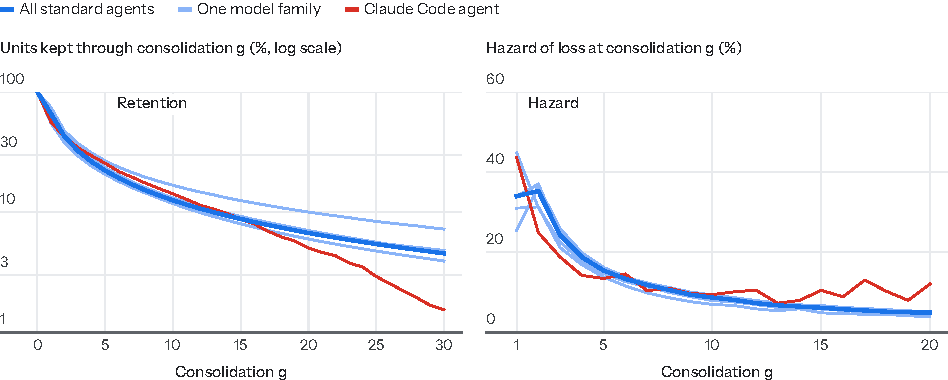
\includegraphics[width=\linewidth]{memory.pdf}
\caption{Fact-unit retention across memory consolidations under literal match. \textbf{a}, Share of units kept through consolidation g on a log axis. \textbf{b}, Hazard of loss at consolidation g. The thick line pools the 45 standard agents, thin blue lines show the four model families and the red line the Claude Code agent. The hazard falls with g in every group.}
\end{figure}

Most of the decline comes from units that differ in durability, and the units that survive also grow safer. As shown in Figure 5, the beta-geometric fit tracks the observed fall in the hazard, and a constant hazard does not. All nine estimates of c′ among survivors lie below 1, between 0.79 and 0.91. Such falling hazards also appear in customer retention and in forgetting curves (Fader and Hardie 2007; Anderson and Tweney 1997; Murre and Chessa 2011).

\begin{figure}[htbp]
\centering
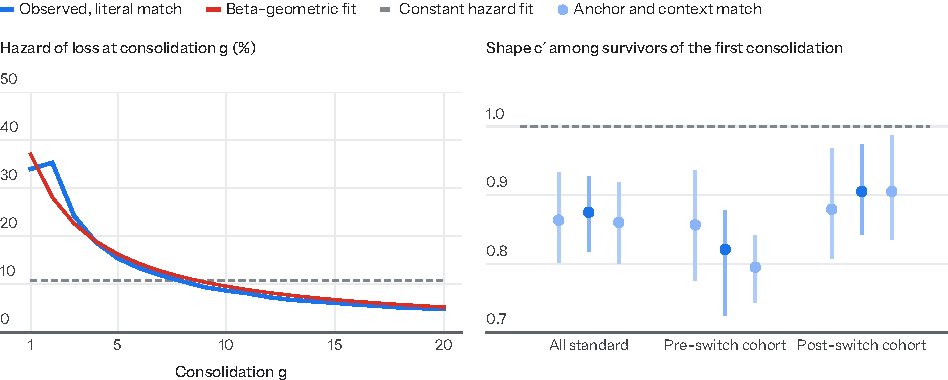
\includegraphics[width=\linewidth]{durability.pdf}
\caption{Durability of fact units under memory consolidation. \textbf{a}, Hazard of loss for all standard agents under literal match, with the constant hazard of the geometric fit and the falling hazard of the beta-geometric fit. \textbf{b}, Beta-discrete-Weibull shape c′ among survivors of the first consolidation for three cohorts under the three presence rules, with 95\% intervals. Units differ in durability, and every c′ below 1 means that survivors also grow safer.}
\end{figure}

The switch to continuous computer use changed when facts are lost. As shown in Figure 6, before the switch a unit is less likely to be lost at its second consolidation than at its first. After the switch it is more likely, by 7.3 points under literal match. Most first losses are drops rather than modifications.

\begin{figure}[htbp]
\centering
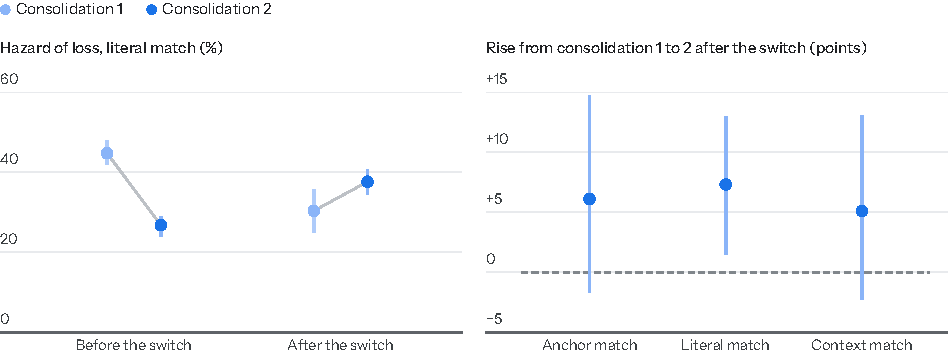
\includegraphics[width=\linewidth]{switch.pdf}
\caption{Hazard of loss at the first two consolidations around the switch to continuous computer use. \textbf{a}, Hazards at consolidations 1 and 2 before and after the switch under literal match, with agent-bootstrap 95\% intervals. \textbf{b}, Paired rise from consolidation 1 to 2 after the switch under the three presence rules. The hazard falls before the switch and rises after it, and only literal match separates the rise from zero.}
\end{figure}

The conclusions hold under all three presence rules, while the magnitudes move with the rule (Table 1). As shown in Figure 7, literal match detects losses with the highest F1 of the three rules against the audit labels, mainly through its precision. Claude agrees with the audit more often than the comparison raters do. Rule-based units still miss format variants, and each miss counts as a loss, so the hazards lean high.

\begin{table}[htbp]
\centering
\small
\caption{Retention under the three presence rules. Hazards are per consolidation with agent-bootstrap intervals. The paired difference is in percentage points with both hazards on the same replicates, and c′ is the beta-discrete-Weibull shape among survivors of the first consolidation.}
\resizebox{\linewidth}{!}{\begin{tabular}{llll}
\toprule
Quantity, 45 standard agents & Anchor match & Literal match & Context match \\
\midrule
Constant hazard rejected in every family & yes & yes & yes \\
h1 & 52.2\% [45.0,~58.1] & 34.0\% [28.9,~38.4] & 46.3\% [39.9,~51.4] \\
h2 & 50.6\% [46.7,~53.7] & 35.3\% [32.5,~37.7] & 43.9\% [40.4,~47.0] \\
h9+ & 4.5\% [3.9,~5.4] & 2.5\% [2.1,~3.0] & 2.5\% [2.2,~2.9] \\
h1 after the switch & 46.6\% [39.4,~53.4] & 30.3\% [24.9,~35.6] & 41.6\% [35.2,~47.6] \\
h2 after the switch & 52.8\% [48.4,~56.3] & 37.6\% [34.3,~40.6] & 46.7\% [42.8,~50.0] \\
h2 − h1 after the switch, paired & +6.1 [−1.7,~+14.8] & +7.3 [+1.5,~+13.0] & +5.1 [−2.3,~+13.1] \\
Modified share of first losses & 23.3\% [20.8,~26.6] & 5.2\% [4.7,~5.6] & 6.6\% [6.0,~7.1] \\
Survivors' c′ & 0.86 [0.80,~0.93] & 0.87 [0.82,~0.93] & 0.86 [0.80,~0.92] \\
Unit-trials & 14,220,326 & 37,881,746 & 25,785,525 \\
\bottomrule
\end{tabular}}
\end{table}

\begin{figure}[htbp]
\centering
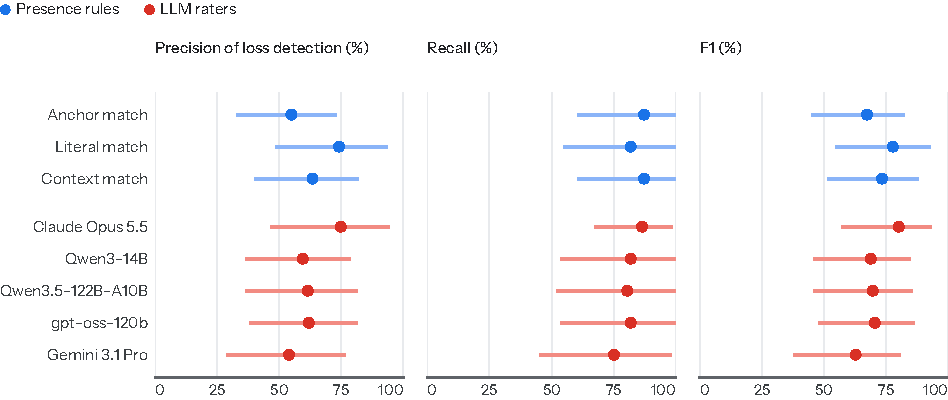
\includegraphics[width=\linewidth]{labels.pdf}
\caption{Precision, recall and F1 of loss detection against the first author's audit labels of 60 units, weighted by inclusion probability, with stratified bootstrap 95\% intervals. Literal match gains precision over anchor match at a similar recall, and Claude Opus 5.5 scores highest among the LLM raters.}
\end{figure}

\section{Retelling between agents}

How far, how fast and how faithfully does information travel from one agent to another?

\subsection{Method}

An information unit collects all occurrences of one anchor across agents in chat messages, search answers and memory versions. A candidate parent must precede an occurrence and be visible to its agent, through its room's chat within three run days, its own memory or its own search answers. The posterior probability that occurrence j is the parent of occurrence i is
\[ P\bigl(\mathrm{parent}(i) = j\bigr) \propto E_{ij}\, K_{ij}\, \exp(\gamma\, S_{ij}), \]
with an exposure indicator $E_{ij}$, a kernel density $K_{ij}$ of log serial intervals and a count $S_{ij}$ of variants that i and j share and the root lacks (Maas 1958). We chose γ~=~0.25 and the time term on 45 occurrences whose parents Claude and the first author labelled.

The most probable parents form the MAP forest (Jombart et al. 2014; Didelot et al. 2017), and generations count transmissions between agents. The headline test uses determined paths, on which every acquisition had a single candidate parent, and compares serial intervals across generations with an Anderson-Darling test under permutations. Intervals run between occurrences in active time, because the logs hold no prompts (Champredon and Dushoff 2015). The content change c is the share of carried quantities whose value changes on an edge.

\subsection{Findings}

Information retold between agents reaches fewer agents than the population allows. As shown in Figure 8, an acquisition in generation 1 leads to 0.235 further acquisitions, half of what the agents that still lack the unit would allow. Later generations reach between a quarter and a third of their expected count. Cause unidentified. Most transmissions go into another agent's memory.

\begin{figure}[htbp]
\centering
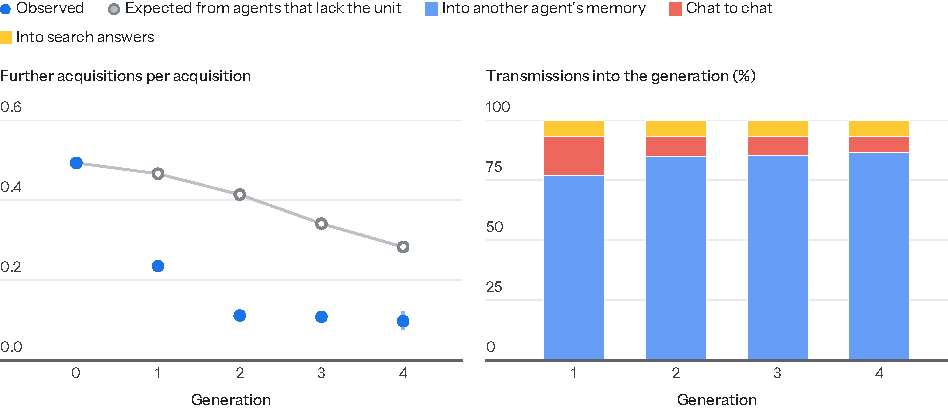
\includegraphics[width=\linewidth]{offspring.pdf}
\caption{Spread of information units between agents on the MAP forest. \textbf{a}, Further acquisitions per acquisition by generation, with root-cluster bootstrap 95\% intervals, against the count expected when the roots' rate scales with the share of agents that still lack the unit. \textbf{b}, Share of transmissions into each generation by channel. From generation 1 on, acquisitions carry between a quarter and a half of the expected count, and most transmissions go into another agent's memory.}
\end{figure}

Information travels more slowly with each retelling. As shown in Figure 9, on determined paths the median serial interval grows with generation in all three channels, with p~=~0.002 in each. The tests reject somewhat too often on synthetic null trees. The same test on the MAP forest rejects far too often and gives no evidence either way.

\begin{figure}[htbp]
\centering
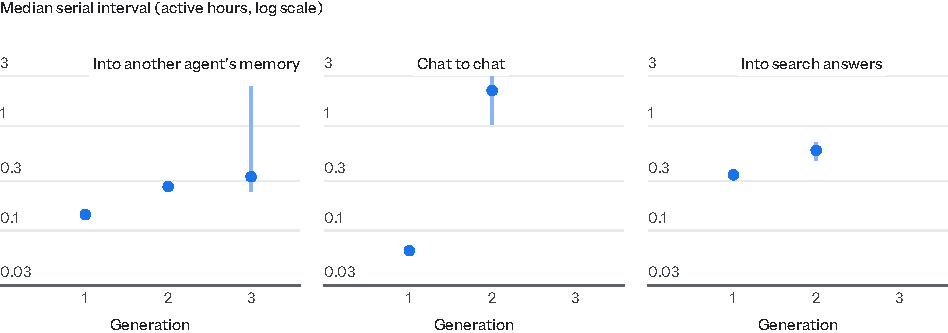
\includegraphics[width=\linewidth]{h1.pdf}
\caption{Median forward serial interval by agent-level generation on determined paths, where every acquisition had a single candidate parent, on a log axis of active hours with 95\% intervals. The interval grows with generation in all three channels, with p~=~0.002 in each.}
\end{figure}

On the MAP forest, the time from a tree root to an acquisition grows faster than linearly with generation. As shown in Figure 10, its mean and variance both rise above the linear trend from the third generation on. Determined paths reach only three generations, and on them the curvature is not distinguishable from zero.

\begin{figure}[htbp]
\centering
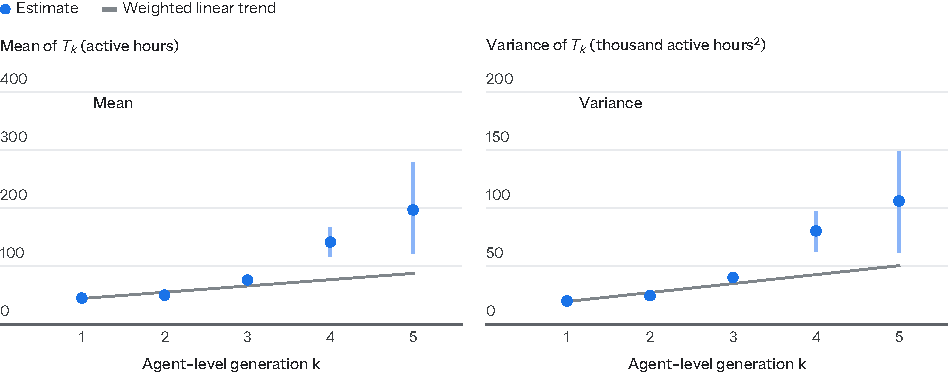
\includegraphics[width=\linewidth]{tk.pdf}
\caption{Mean and variance of $T_k$, the active time from a tree root to an acquisition at agent-level generation k on the MAP forest. Intervals are root-cluster bootstrap 95\% intervals, and the line is the weighted linear trend in k. From k~=~3 on, both estimates and their whole intervals lie above the linear trend.}
\end{figure}

Retelling changes values more often than memory consolidation does. As shown in Figure 11, 30.1\% of quantities carried from one agent to another change value, against at most 13.0\% in a consolidation under any presence rule. Chat between agents changes values most often. Children of a changed node keep the new value about as often as they return to the old one. Wording drifts toward a common form, as in iterated LLM transmission (Perez et al. 2025).

\begin{figure}[htbp]
\centering
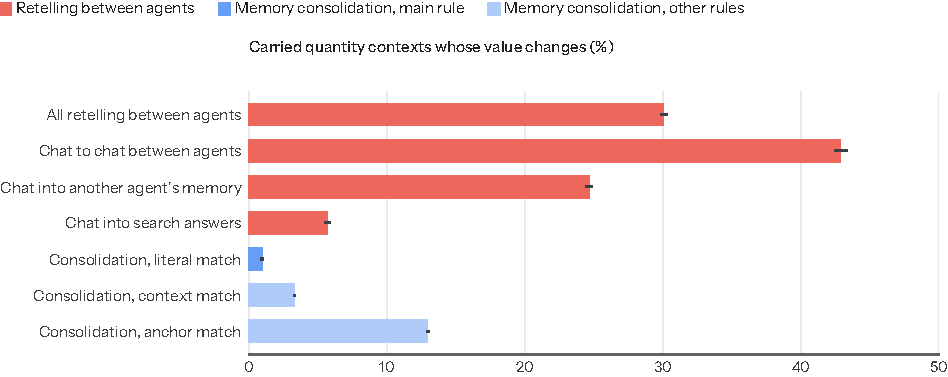
\includegraphics[width=\linewidth]{h3.pdf}
\caption{Share of carried quantity contexts whose value changes, by channel of retelling between agents and for memory consolidation under the three presence rules, with 95\% intervals. Retelling changes values more often than consolidation under every rule.}
\end{figure}

The determined paths are reliable on synthetic trees, where 95.4\% of their parents are correct, against 79.2\% for MAP parents. The parent posterior rests on few labels, and simple recency rules match them at least as well, so results that depend on it describe the MAP forest only.

\section{Shared work}

Whose earlier work does each computer-use session build on?

\subsection{Method}

Nodes are the 78,362 computer-use sessions, and artifacts are documents, code paths, URLs and files. Touch rules classify each step's contact with an artifact as a write or a read. Session A is a parent of session B when A was the last other session to write an artifact before B first touched it. We build one graph per village goal and place each session one layer below its deepest parent.

We compare these graphs with a generative model of swarm work that the toolkit implements. The model grows a task DAG layer by layer, with layer widths that rise to a peak early in the DAG and then taper. Each new step takes a main parent in the layer above, preferring parents that improved on their own best parent, and about half of the steps also merge extra parents. A step at depth d of a DAG with D layers costs \texttt{c\_d}~=~1 + 9d/(D − 1), so the deepest steps cost ten times the root. Agents work through the DAG alone, in a standard swarm that a coordinator keeps at N agents, or in a recursive swarm whose agents fork sub-agents. The generator gives 64 DAGs per goal with as many steps as the goal has sessions. The continuation rate is the share of consecutive session pairs of one agent in which the earlier session is a parent of the later one. Figure 12 shows the graph of one goal next to a generator DAG of the same size.

\begin{figure}[htbp]
\centering
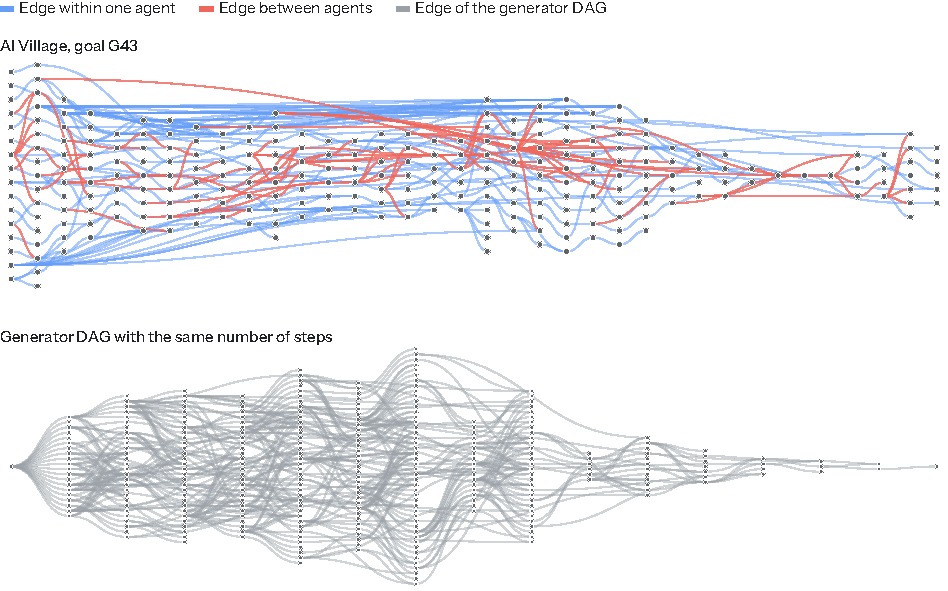
\includegraphics[width=\linewidth]{depgraph_example.pdf}
\caption{Dependency graphs drawn layer by layer from left to right. \textbf{a}, Goal G43 of the AI Village, leaving out sessions without any edge. Blue edges join two sessions of one agent, and red edges join sessions of different agents. \textbf{b}, A DAG from the generator with as many steps as the goal has sessions. Most edges of the real graph stay within one agent, and far more of them skip layers than in the generator.}
\end{figure}

\subsection{Findings}

Agents mostly continue their own previous session. As shown in Figure 13, the earlier session is a parent in 60.2\% of 50,251 consecutive pairs, against at most 25.0\% for random parents. The rate rises after the switch to continuous computer use.

\begin{figure}[htbp]
\centering
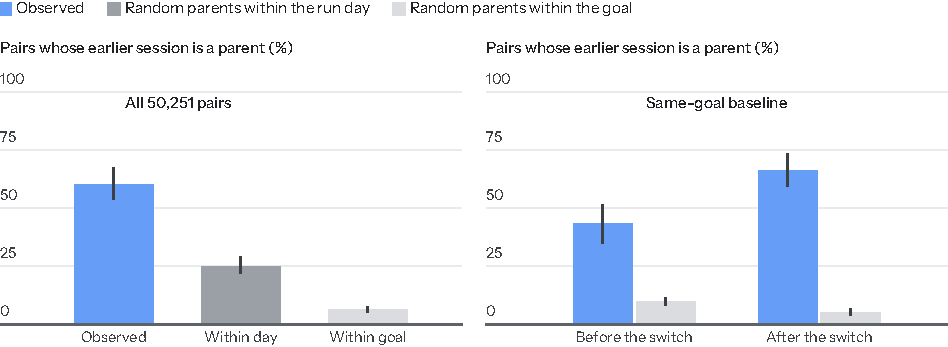
\includegraphics[width=\linewidth]{continuation.pdf}
\caption{Share of consecutive session pairs of one agent in which the earlier session is a parent of the later one, with agent-bootstrap 95\% intervals. Baselines draw random parents from artifacts written earlier in the same run day or goal. \textbf{a}, All 50,251 pairs. \textbf{b}, Pairs before and after the switch to continuous computer use, against the same-goal baseline. Agents continue their own previous session far more often than chance.}
\end{figure}

Real task graphs are denser than the generator's. As shown in Figure 14, a step has more parents and far more edges skip layers, while children spread more evenly. Five of the six statistics lie outside the range of 64 generator replicates.

\begin{figure}[htbp]
\centering
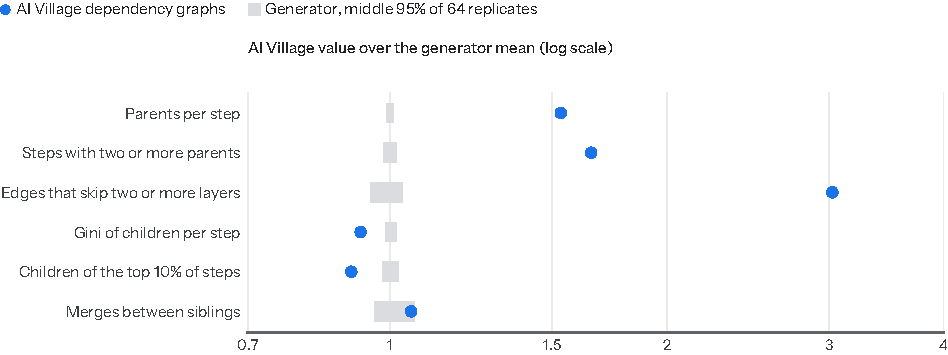
\includegraphics[width=\linewidth]{structure.pdf}
\caption{Six structure statistics of the AI Village dependency graphs over the generator mean, on a log axis, for all edges under touch rules v2 pooled over 51 goals. Bars span the middle 95\% of 64 generator replicates. Real graphs have more parents per step and far more edges that skip layers.}
\end{figure}

Step cost does not grow with depth. As shown in Figure 15, sessions deep in a goal's graph take about as many turns and active minutes as those at its start. The model's cost \texttt{c\_d} rises about ninefold.

\begin{figure}[htbp]
\centering
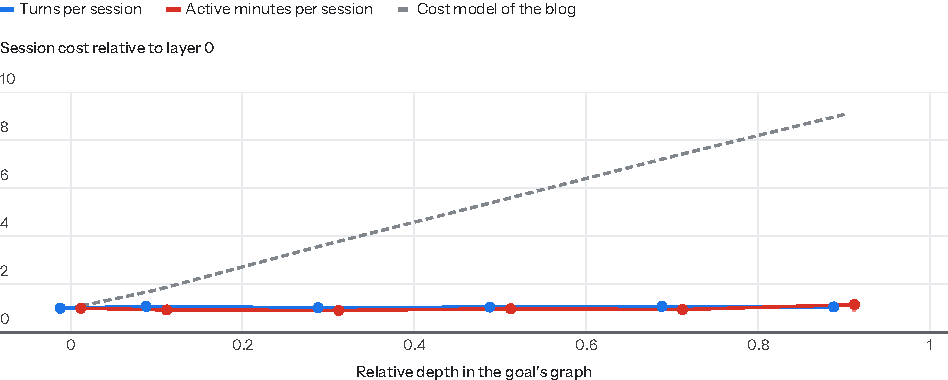
\includegraphics[width=\linewidth]{stepcost.pdf}
\caption{Turns and active minutes per computer-use session relative to the goal's layer-0 sessions, by relative depth in the goal's dependency graph, with 95\% intervals, against the cost \texttt{c\_d} of the model. Real sessions cost about the same at every depth, while the cost model rises about ninefold.}
\end{figure}

The simulator shows how swarms speed up work on DAGs like these. As shown in Figure 16, a standard swarm of 64 agents covers half of a DAG 31.7 times faster than one agent. The scaling exponent ln g / ln N, with g the speedup to half coverage, stays between 0.83 and 0.93 for both swarm types at every checked size. All 15 checks against the reference values of the model's first implementation pass within 20\% without tuning. The conclusions on the AI Village graphs also hold on the goals where most GUI writes can be traced to an artifact.

\begin{figure}[htbp]
\centering
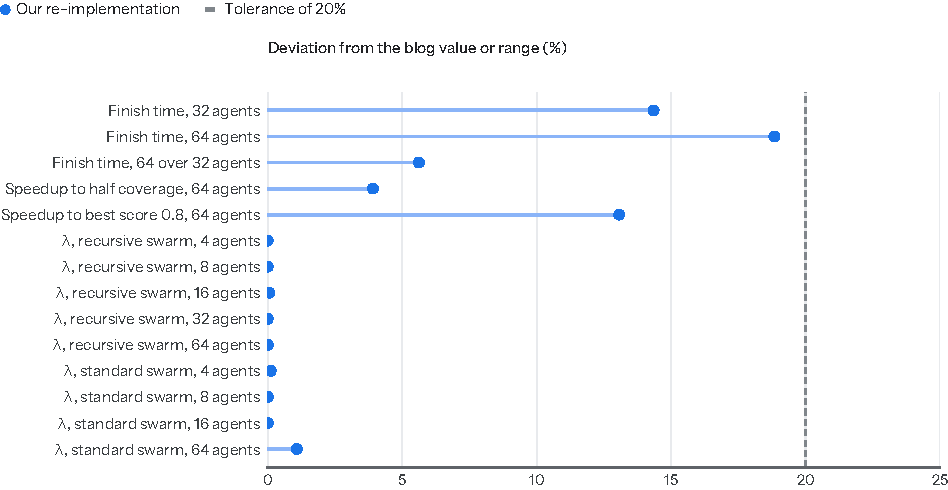
\includegraphics[width=\linewidth]{reproduction.pdf}
\caption{Deviation of the simulator from the reference values of the model for the 14 quantitative checks, relative to the reference value or the nearest end of a reference range, over 256 families of 16 tasks. The fifteenth check, earlier coverage at every larger swarm, holds in all 256 families. Every deviation stays below the 20\% tolerance.}
\end{figure}

\section{Scaffolding changes}

Do documented changes to the scaffold shift behaviour?

\subsection{Method}

We detect change points in 387 behavioural series, such as the message counts, waits, sessions and search calls of model families, single agents and word groups. PELT finds them (Killick, Fearnhead and Eckley 2012; Truong, Oudre and Vayatis 2020), and BOCPD checks them (Adams and MacKay 2007). We count change points within three run days of a CHANGELOG entry. Nulls that move the entries at random give the count expected by chance, and some of them keep each entry on its weekday. A change point with no documented event nearby is labelled cause unidentified.

\subsection{Findings}

Change points do not line up with CHANGELOG entries beyond chance. As shown in Figure 17, 1,929 of 2,314 change points lie near an entry, close to the 1,969.5 expected by chance, p~=~0.695. Entries are so dense that most run days lie near one, so the test has little power.

\begin{figure}[htbp]
\centering
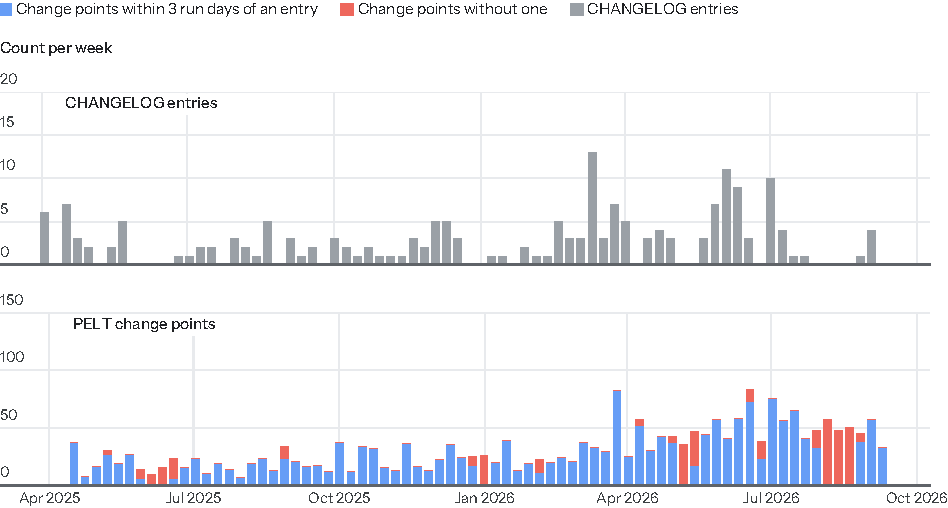
\includegraphics[width=\linewidth]{changepoints.pdf}
\caption{Weekly counts of CHANGELOG entries and of PELT l2 change points in 387 series from April 2025 to September 2026. Blue change points have an entry within three run days, and red ones do not. Entries are dense enough that most change points sit near one.}
\end{figure}

Change points cluster at goal transitions and at week starts, and the data cannot separate the two. As shown in Figure 18, a third of the change points of daily series fall on Mondays, and 39 of the 51 goal transitions start on a Monday. Of all change points, 208 have no documented event within three run days, most of them between late July and late August 2026. Cause unidentified.

\begin{figure}[htbp]
\centering
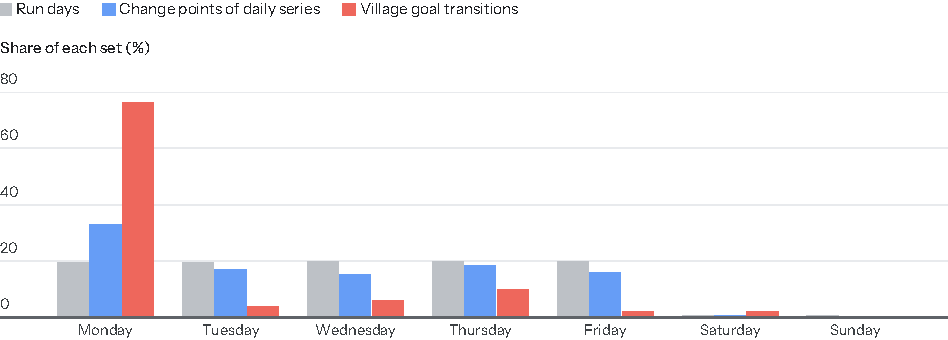
\includegraphics[width=\linewidth]{weekdays.pdf}
\caption{Weekday shares of the 389 run days, of the 1,543 PELT l2 change points of daily series and of the 51 village goal transitions. Change points and goal transitions both concentrate on Mondays.}
\end{figure}

\section{Limitations}

The excitation model fits the timing of single agents poorly, and its explicit-reference check falls below a simple baseline. The LLM monitor is not ground truth, so agreement with it only shows consistency between two readings. Rule-based fact units miss format variants, and each miss biases the memory hazards upward. The logs hold no prompts, so we measure serial intervals between occurrences instead of generation intervals between exposures. The parent posterior rests on few labels. GUI work before October 2025 leaves few traceable artifacts, and the screenshots could recover them. All results come from one community of agents under one evolving scaffold.

\section{Reproducibility}

Every step reads \texttt{configs/\allowbreak{}default.\allowbreak{}yaml}. It pins the dataset revision and the seed 20261003 for every stochastic step. All steps run as CPU jobs under Slurm, local LLM labelling used vLLM on GPU nodes, and no paid API was called. Table A11 lists the commands in run order with their runtimes. The label sheets hold personal data and stay private.

\section*{Acknowledgments}

We thank AI Digest for the AI Village dataset and the public monitor findings. Please cite the data as AI Digest, ``AI Village dataset'', 2026, \url{https://theaidigest.org/village}.

\section*{References}

\begin{itemize}[leftmargin=1.5em, itemsep=1pt, parsep=0pt, label={}]
\small
\item Adams and MacKay. 2007. Bayesian online changepoint detection. arXiv:0710.3742.
\item AI Digest. 2026. AI Village dataset. \url{https://theaidigest.org/village}. Hugging Face dataset aidigestorg/ai-village, revision \texttt{838b415030\allowbreak{}3ca8228e8e\allowbreak{}db432d8b8c\allowbreak{}cae353d258}.
\item Anderson and Tweney. 1997. Artifactual power curves in forgetting. Memory and Cognition 25(5), 724-730. doi:10.3758/BF03211315.
\item Binksmith. 2026-06-16. How the AI Village works. \url{https://aivillageblog.substack.com/p/how-the-ai-village-works}
\item Brown et al. 2002. The time-rescaling theorem and its application to neural spike train data analysis. Neural Computation.
\item Champredon and Dushoff. 2015. Intrinsic and realized generation intervals in infectious-disease transmission. Proceedings of the Royal Society B.
\item Didelot et al. 2017. Genomic infectious disease epidemiology in partially sampled and ongoing outbreaks. Molecular Biology and Evolution.
\item Fader and Hardie. 2007. How to project customer retention. Journal of Interactive Marketing 21(1). \url{https://onlinelibrary.wiley.com/doi/abs/10.1002/dir.20074}
\item Fader, Hardie, Liu, Davin and Steenburgh. 2018. ``How to Project Customer Retention'' Revisited: The Role of Duration Dependence. Journal of Interactive Marketing 43(1), 1-16. doi:\texttt{10.\allowbreak{}1016/\allowbreak{}j.\allowbreak{}intmar.\allowbreak{}2018.\allowbreak{}01.\allowbreak{}002}.
\item Heckman and Singer. 1984. A Method for Minimizing the Impact of Distributional Assumptions in Econometric Models for Duration Data. Econometrica 52(2), 271-320. doi:10.2307/1911491.
\item Jombart et al. 2014. Bayesian reconstruction of disease outbreaks by combining epidemiologic and genomic data. PLoS Computational Biology.
\item Killick, Fearnhead and Eckley. 2012. Optimal detection of changepoints with a linear computational cost. JASA.
\item Maas. 1958. Textual Criticism.
\item Murre and Chessa. 2011. Power laws from individual differences in learning and forgetting: mathematical analyses. Psychonomic Bulletin and Review 18, 592-597.
\item Perez et al. 2025. When LLMs Play the Telephone Game: Cumulative Changes and Attractors in Iterated Cultural Transmissions. ICLR 2025. arXiv:2407.04503.
\item Truong, Oudre and Vayatis. 2020. Selective review of offline change point detection methods. Signal Processing.
\item Vaupel, Manton and Stallard. 1979. The impact of heterogeneity in individual frailty on the dynamics of mortality. Demography 16(3), 439-454. doi:10.2307/2061224.
\item Vaupel and Yashin. 1985. Heterogeneity's Ruses: Some Surprising Effects of Selection on Population Dynamics. The American Statistician 39(3), 176-185. doi:\texttt{10.\allowbreak{}1080/\allowbreak{}00031305.\allowbreak{}1985.\allowbreak{}10479424}.
\item Veen and Schoenberg. 2008. Estimation of space-time branching process models in seismology using an EM-type algorithm. JASA.
\item Weinberg and Gladen. 1986. The Beta-Geometric Distribution Applied to Comparative Fecundability Studies. Biometrics 42(3), 547-560. doi:10.2307/2531205.
\end{itemize}

\appendix
\section{Supplementary tables}
\renewcommand{\thetable}{A\arabic{table}}\setcounter{table}{0}

These tables give the size of each source table, the values behind Figures 9, 11, 13, 15 and 16, the change-point counts of Section 7, further checks of the excitation model and the commands that reproduce every result.

\begin{table}[htbp]
\centering
\small
\caption{Rows per table at revision 838b4150 against the dataset card. Every count equals the export manifest, with no duplicate id and no unparsed timestamp.}
\begin{tabular}{lrr}
\toprule
Table & Rows & Dataset card \\
\midrule
events & 381,610 & $\approx$233,000 \\
\texttt{chat\_messages} & 183,485 & $\approx$123,000 \\
\texttt{computer\_use\_sessions} & 78,362 & $\approx$37,000 \\
\texttt{computer\_use\_turns} & 2,510,487 & $\approx$1,140,000 \\
\texttt{agent\_memories} & 246,151 & $\approx$165,000 \\
summaries & 939 & $\approx$800 \\
\texttt{claude\_code\_messages} & 244,820 & $\approx$245,000 \\
\texttt{claude\_code\_sessions} & 303 & $\approx$300 \\
agents & 46 & 31 \\
\texttt{chat\_rooms} & 16 & 5 \\
\texttt{village\_goals} & 51 & $\approx$45 \\
\texttt{agent\_goals} & 33 & not listed \\
villages & 1 & 1 \\
\bottomrule
\end{tabular}
\end{table}

\begin{table}[htbp]
\centering
\small
\caption{Serial intervals by generation on determined paths, where every acquisition from the root had a single candidate parent. Medians are forward serial intervals, and p comes from 499 permutations. The type I error is the rejection rate on 100 synthetic null replicates, and the power the rejection rate on 25 replicates with 1.5-fold growth per generation.}
\resizebox{\linewidth}{!}{\begin{tabular}{llrllll}
\toprule
Stratum & Generation & Transmissions & Median, active h [95\% CI] & Test p & Type I error & Power \\
\midrule
Chat to another agent's memory & 1 & 347,801 & 0.142 [0.141,~0.143] & 0.002 & 7.0\% [3.4,~13.7] & 100\% [87,~100] \\
 & 2 & 3,993 & 0.263 [0.237,~0.289] &  &  &  \\
 & 3 & 69 & 0.326 [0.237,~2.375] &  &  &  \\
Chat to chat, between agents & 1 & 84,450 & 0.064 [0.063,~0.065] & 0.002 & 13.0\% [7.8,~21.0] & 40\% [23,~59] \\
 & 2 & 407 & 2.17 [1.04,~3.82] &  &  &  \\
Chat to search answer & 1 & 25,558 & 0.340 [0.331,~0.365] & 0.002 & not simulated & not simulated \\
 & 2 & 758 & 0.582 [0.464,~0.687] &  &  &  \\
\bottomrule
\end{tabular}}
\end{table}

\begin{table}[htbp]
\centering
\small
\caption{Content change, the share of carried quantity contexts whose value changes. Retelling intervals come from a root-cluster bootstrap, and the consolidation rows use a Wilson interval that ignores clustering by agent.}
\begin{tabularx}{\linewidth}{Lrl}
\toprule
Channel & Contexts & c [95\% CI] \\
\midrule
All retelling between agents & 909,623 & 30.1\% [29.9,~30.2] \\
Chat to chat, between agents & 269,365 & 42.9\% [42.5,~43.3] \\
Chat to another agent's memory & 640,258 & 24.7\% [24.5,~24.8] \\
Chat to search answer & 255,850 & 5.7\% [5.5,~5.8] \\
Memory consolidation, quantities, literal match & 19,437,527 & 0.95\% [0.95,~0.96] \\
Memory consolidation, quantities, anchor match & 6,550,788 & 13.0\% [12.9,~13.0] \\
Memory consolidation, quantities, context match & 7,386,947 & 3.3\% [3.3,~3.3] \\
\bottomrule
\end{tabularx}
\end{table}

\begin{table}[htbp]
\centering
\small
\caption{Step cost by depth and continuation of an agent's previous session. Slope intervals resample 49 goals, continuation intervals resample agents, and the switch rows use the same-goal baseline.}
\resizebox{\linewidth}{!}{\begin{tabular}{llll}
\toprule
Quantity & Estimate [95\% CI] & Reference [95\% CI] & n \\
\midrule
Slope of relative turns on depth & 0.029 [−0.092,~0.074] & 9 in the model & 77,725 sessions \\
Slope of relative active minutes & 0.151 [−0.122,~0.255] & 9 in the model & 77,725 sessions \\
Continuation, same-goal baseline & 60.2\% [53.4,~67.4] & 6.3\% [5.1,~7.7] & 50,251 pairs \\
Continuation, same-day baseline & 60.2\% [53.6,~67.3] & 25.0\% [21.8,~29.0] & 50,251 pairs \\
Continuation before the switch & 43.2\% [34.7,~51.6] & 9.6\% [7.9,~11.3] & 12,733 pairs \\
Continuation after the switch & 66.0\% [59.1,~73.4] & 5.2\% [3.9,~6.6] & 37,516 pairs \\
\bottomrule
\end{tabular}}
\end{table}

\begin{table}[htbp]
\centering
\small
\caption{Alignment of PELT l2 change points with goal events and CHANGELOG entries, unadjusted p. Null 2 places entries uniformly over run days, and null 2w keeps each entry on its own weekday.}
\begin{tabular}{llrll}
\toprule
Entry set & w & Aligned of 2,314 & Null 2 p & Null 2w p \\
\midrule
Village goal transitions & 0 & 877 & < 0.001 & 0.005 \\
Village goal transitions & 1 & 1,240 & 0.003 & 0.269 \\
CHANGELOG goal category & 0 & 315 & 0.001 & 0.002 \\
CHANGELOG goal category & 1 & 474 & 0.031 & 0.039 \\
All CHANGELOG entries & 0 & 1,235 & 0.055 & 0.081 \\
All CHANGELOG entries & 3 & 1,929 & 0.998 & 0.998 \\
\bottomrule
\end{tabular}
\end{table}

\begin{table}[htbp]
\centering
\small
\caption{PELT l2 change points without a documented cause by series level. Documented events are CHANGELOG entries, village goal transitions and the series' own agent goal changes.}
\begin{tabular}{lrrr}
\toprule
Level & Change points & No CHANGELOG entry within 3 run days & No documented event \\
\midrule
Agent & 1,105 & 238 & 147 \\
Family & 584 & 79 & 33 \\
Lexical & 625 & 68 & 28 \\
All & 2,314 & 385 & 208 \\
\bottomrule
\end{tabular}
\end{table}

\begin{table}[htbp]
\centering
\small
\caption{Further checks of the excitation model. Intervals come from a run-day cluster bootstrap, and the time-rescaling test joins each agent's present days end to end.}
\begin{tabularx}{\linewidth}{lLLl}
\toprule
Aspect & Check & Result & n \\
\midrule
Timing & Time-rescaling KS test at 5\% & 68\% of dimensions reject & 393 dimensions \\
Parents & Most probable parent equals the label & 15.0\% [14.0,~16.0] & 16,851 children \\
Parents & Latest message by someone else & 34.3\% [32.1,~36.7] & 16,851 children \\
Parents & Most probable parent among other speakers & 38.6\% [37.1,~40.5] & 16,851 children \\
Rankings & Spearman of opportunity and Hawkes rankings & median 0.128 [0.072,~0.187], negative in 8 & 43 windows \\
Sensitivity & Largest share change, L of 1 or 6 h & 7.1\% & 43 windows \\
Sensitivity & Largest change in ρ, L of 1 h & 0.198 & 43 windows \\
\bottomrule
\end{tabularx}
\end{table}

\begin{table}[htbp]
\centering
\small
\caption{The excitation model against the LLM monitor. Share rows are differences in posterior parent-class shares between messages near a finding and the same agents' other messages. Percentile rows rank flagged pairs among all pairs of a window, where 50 is chance.}
\resizebox{\linewidth}{!}{\begin{tabular}{llll}
\toprule
Reading & Subset & Estimate [95\% CI] & n \\
\midrule
Self share, flagged minus control & all findings & +3.9\% [2.6,~5.2] & 21,184 flagged messages \\
Self share, same hour of run & all findings & +2.8\% [1.7,~4.0] & 10,383 flagged messages \\
Other-agent share & all findings & −2.0\% [−2.6,~−1.3] & 21,184 flagged messages \\
Other-agent share, same hour of run & all findings & −0.5\% [−1.3,~0.5] & 10,383 flagged messages \\
Share on agents named in the conflict & conflicts & +0.9\% [0.3,~1.4] & 1,956 flagged messages \\
Mean percentile of $n_{ij} + n_{ji}$ & conflict pairs & 62.0 [54.7,~68.1] & 299 pairs \\
Mean percentile of $n_{ij} + n_{ji}$ & all flagged pairs & 64.6 [60.9,~65.6] & 4,811 pairs \\
Percentile, once per distinct pair & conflict pairs & 55.9 [49.9,~61.1] & 121 pairs \\
Percentile, once per distinct pair & all flagged pairs & 52.0 [49.9,~54.7] & 595 pairs \\
\bottomrule
\end{tabular}}
\end{table}

\begin{table}[htbp]
\centering
\small
\caption{The 15 checks of the simulator against the reference values of the model, with λ rows grouped by swarm size. Deviation is relative to the reference value or to the nearest end of a reference range, and the tolerance is 20\%.}
\resizebox{\linewidth}{!}{\begin{tabular}{llll}
\toprule
Check & Reference & Simulator [95\% CI] & Deviation \\
\midrule
Coverage earlier at every larger swarm & yes & 256 of 256 families & none \\
Speedup to half coverage, 64 agents & 33 & 31.7 [31.5,~31.9] & 3.9\% \\
Speedup to best score 0.8, 64 agents & 16 & 18.1 [17.8,~18.4] & 13.1\% \\
Finish time, 32 agents, in T₁ & about 0.10 & 0.086 [0.083,~0.088] & 14.4\% \\
Finish time, 64 agents, in T₁ & about 0.10 & 0.081 [0.079,~0.084] & 18.8\% \\
Finish time, 64 over 32 agents & about 1 & 0.944 [0.936,~0.951] & 5.6\% \\
λ, standard swarm, 4 to 16 agents & 0.89 to 0.92 & 0.889 to 0.914 & at most 0.1\% \\
λ, standard swarm, 64 agents & 0.84 & 0.831 [0.830,~0.832] & 1.1\% \\
λ, recursive swarm, 4 to 64 agents & 0.88 to 0.93 & 0.885 to 0.931 & at most 0.1\% \\
\bottomrule
\end{tabular}}
\end{table}

\begin{table}[htbp]
\centering
\small
\caption{Structure and continuation on subsets of goals with a small GUI focus gap, touch rules v2. Generator columns give the mean of 64 replicates, and every observed value lies above the generator's 97.5th percentile.}
\resizebox{\linewidth}{!}{\begin{tabular}{lrrrrrl}
\toprule
Subset & Goals & Mean parents & Generator & Layer-skipping edges & Generator & Continuation [95\% CI] \\
\midrule
All goals & 51 & 2.67 & 1.74 & 60.0\% & 19.8\% & 60.2\% [53.5,~67.2] \\
Gap below 20\% & 24 & 2.74 & 1.74 & 60.9\% & 20.1\% & 62.7\% [55.7,~69.7] \\
Gap below 10\% & 13 & 2.88 & 1.74 & 62.7\% & 20.3\% & 66.7\% [59.2,~74.1] \\
Touch share at least 80\% & 17 & 2.07 & 1.73 & 48.1\% & 19.2\% & 58.3\% [52.1,~65.8] \\
Goals from 2025-10 & 36 & 2.68 & 1.74 & 60.2\% & 19.9\% & 60.9\% [54.4,~68.1] \\
Without GUI-heavy early goals & 40 & 2.68 & 1.74 & 60.1\% & 19.9\% & 60.7\% [54.0,~67.5] \\
\bottomrule
\end{tabular}}
\end{table}

\begin{table}[htbp]
\centering
\small
\caption{Commands in run order. Change-point detection reads the outputs of the excitation model, the memory step and the monitor, and the transmission trees read the excitation-model kernels. In the memory step the default run gives anchor match, \texttt{--rules v2} gives literal match and \texttt{--rules v3} gives context match.}
\begin{tabularx}{\linewidth}{lLL}
\toprule
Step & Command & Runtime \\
\midrule
Ingest & \texttt{avsd ingest} & about 5 min, 8 CPUs \\
Event table & \texttt{avsd build-\allowbreak{}events} & 55 s, 8.7 GB peak memory \\
Excitation model & \texttt{avsd hawkes fit --window goal}, then \texttt{--window rolling} & acceptance 224 s, bootstrap shards of 605 to 2,368 s, matched arms 1,055 s and 1,066 s, 16 workers each \\
Monitor & \texttt{run\_\allowbreak{}monitor\_\allowbreak{}ingest} in \texttt{avsd.\allowbreak{}validate.\allowbreak{}monitor}, then \texttt{python -m avsd.\allowbreak{}validate.\allowbreak{}monitor\_\allowbreak{}hawkes} & fetch about 22 min, validation 14 s \\
Memory retention & \texttt{avsd lineage memory}, then \texttt{python -m avsd.\allowbreak{}lineage.\allowbreak{}memory --rules v2} and \texttt{--rules v3}, then \texttt{python scripts/\allowbreak{}b1\_\allowbreak{}post\_\allowbreak{}switch\_\allowbreak{}rise.\allowbreak{}py} & 687 s, 1,214 s and 1,900 s from the anchor cache, plus 1,555 s for the first extraction and about 1 min for the paired test \\
Transmission trees & \texttt{python -m avsd.\allowbreak{}lineage.\allowbreak{}b2\_\allowbreak{}units}, then \texttt{avsd lineage trees --gamma composite} & 24 min on 48 CPUs, then 1,577 s \\
Change points & \texttt{avsd changepoint} & 144 s, 16 processes \\
Simulator & \texttt{avsd swarmsim reproduce} & 77 s, 32 processes \\
Dependency graphs & \texttt{avsd swarmsim calibrate}, then \texttt{--rules v1}, then \texttt{python scripts/\allowbreak{}depgraph\_\allowbreak{}example.\allowbreak{}py} & 109 s and 108 s, 48 processes, plus about 2 min of touch extraction and 14 s for the example graph \\
Report & \texttt{avsd report} & 78 s \\
\bottomrule
\end{tabularx}
\end{table}

\end{document}
